\documentclass[aspectratio=169]{beamer}

\usetheme{GRVC}

% --- Timeline styles/macro (works in presentation + handout) ---
\usepackage{tikz}
\usetikzlibrary{arrows,calc,positioning,shadows}
\tikzset{>=stealth'}

\definecolor{TLaxis}{RGB}{235,235,235}
\definecolor{TLorange}{RGB}{241,120,0}
\definecolor{TLblue}{RGB}{0,145,220}
\definecolor{TLgreen}{RGB}{70,170,0}

\tikzset{
	tlAxis/.style={draw=TLaxis, line width=2.2pt, line cap=round},
	tlMajorTick/.style={draw=TLaxis, line width=1.0pt},
	tlMinorTick/.style={draw=TLaxis, line width=0.55pt},
	tlMonth/.style={font=\scriptsize, text=TLaxis},
	tlYear/.style={font=\bfseries\small, text=TLaxis},
	tlConn/.style={densely dashed, line width=0.9pt},
	tlBox/.style={
		rounded corners=2pt,
		align=left,
		text=white,
		font=\tiny,
		inner xsep=6pt,
		inner ysep=5pt,
		fill opacity=0.92,
		draw opacity=0.92,
		line width=0.6pt,
		drop shadow={opacity=0.25}
	},
	tlOrange/.style={tlBox, fill=TLorange, draw=TLorange},
	tlBlue/.style={tlBox, fill=TLblue, draw=TLblue},
	tlGreen/.style={tlBox, fill=TLgreen, draw=TLgreen},
}

\newcommand{\TLAbove}[5]{% x, y, boxstyle, color, text
	\coordinate (TLp) at (#1,0);
	\fill[#4] (TLp) circle (2.0pt);
	\draw[#4, line width=0.8pt] (TLp) circle (2.9pt);
	\node[#3] (TLb) at (#1,#2) {#5};
	\path[fill=#4, draw=#4, line width=0.6pt]
	($(TLb.south)+(-0.35,0)$) --
	($(TLb.south)+( 0.35,0)$) --
	($(TLb.south)+( 0,-0.33)$) -- cycle;
	\draw[tlConn, color=#4] (TLp) -- ($(TLb.south)+(0,-0.33)$);
}

\newcommand{\TLBelow}[5]{% x, y, boxstyle, color, text
	\coordinate (TLp) at (#1,0);
	\fill[#4] (TLp) circle (2.0pt);
	\draw[#4, line width=0.8pt] (TLp) circle (2.9pt);
	\node[#3] (TLb) at (#1,#2) {#5};
	\path[fill=#4, draw=#4, line width=0.6pt]
	($(TLb.north)+(-0.35,0)$) --
	($(TLb.north)+( 0.35,0)$) --
	($(TLb.north)+( 0, 0.33)$) -- cycle;
	\draw[tlConn, color=#4] (TLp) -- ($(TLb.north)+(0,0.33)$);
}


% Blocks
\setbeamerfont{block title}{size=\normalsize, series=\bfseries}
\setbeamerfont{block body}{size=\small}

% Itemize / enumerate
\setbeamerfont{itemize/enumerate body}{size=\small}
\setbeamerfont{itemize/enumerate subbody}{size=\footnotesize}


\usepackage{tikz}
\usetikzlibrary{calc}

% Partner logo helper (used for consortium slides)
\newcommand{\GRVCpartnerlogo}[1]{%
  \includegraphics[width=0.16\textwidth,height=1.5cm,keepaspectratio]{#1}%
}

% Set a transparent background image for all frames
\setbeamertemplate{background}{%
  \begin{tikzpicture}[remember picture,overlay]
    \node[opacity=0.95, at=(current page.center)] {%
      \includegraphics[width=\paperwidth,height=\paperheight]{assets/background.png}%
    };
  \end{tikzpicture}%
}

\title{GRVC Lab\\Biweekly seminars}
\author{Abdalraheem Abdullah Yousef Ijieh}
% \institute{GRVC Robotics Labs}
\date{16 Enero 2026}

\begin{document}

% Title slide (first slide) includes GRVC logo at lower-left by design
\begin{frame}[plain]
  \titlepage
\end{frame}


% Example: section divider with project logo (top-right)
\GRVCsectionframe[assets/tema\_logo.png]{Trusted extremely precise mapping and prediction for emergency management}

% --- Consortium partners (logos are sourced from the official TEMA partners page) ---
{\setbeamertemplate{background}{%
  \begin{tikzpicture}[remember picture,overlay]
    \fill[GRVCCYAN] (current page.south west) rectangle (current page.north east);
  \end{tikzpicture}}
  }


{
\GRVCsetprojectlogo{assets/tema_logo.pdf}

% ============================================================
% Roadmap (fixes pacing and expectations)
% ============================================================
\begin{frame}{Roadmap}
	\small
	\begin{enumerate}\itemsep0.5em
		\item TEMA context: partners and technologies (USE scope)
		\item PDM-tech-05: Information Fusion platform (problem \textrightarrow{} approach \textrightarrow{} outputs)
		\item Fusion methods: OGM (hazard occupancy) and OPM (multi-object tracking)
		\item Flood case study (Ahrtal): inputs, fusion evolution, outputs and lessons learned
	\end{enumerate}
\end{frame}

\begin{frame}{TEMA in a Nutshell}
  \begin{columns}[T,onlytextwidth]
    % ---------------- Left column: Partners ----------------
    \column{0.4\textwidth}
      \centering
      {\bfseries Consortium partners}\par\vspace{0.4em}

      % tighten spacing so it fits nicely
      \setlength{\tabcolsep}{3pt}
      \renewcommand{\arraystretch}{0.95}

      \begin{tabular}{ccccc}
        \GRVCpartnerlogo{assets/partners/auth.png} &
        \GRVCpartnerlogo{assets/partners/atos.png} &
        \GRVCpartnerlogo{assets/partners/brk.png} &
        \GRVCpartnerlogo{assets/partners/dmalian.png} &
        \GRVCpartnerlogo{assets/partners/engineering.png} \\
        \GRVCpartnerlogo{assets/partners/fraunhofer_hhi.png} &
        \GRVCpartnerlogo{assets/partners/dlr.png} &
        \GRVCpartnerlogo{assets/partners/itu.png} &
        \GRVCpartnerlogo{assets/partners/kamk.png} &
        \GRVCpartnerlogo{assets/partners/kaj.png} \\
        \GRVCpartnerlogo{assets/partners/kemea.png} &
        \GRVCpartnerlogo{assets/partners/latitudo40.png} &
        \GRVCpartnerlogo{assets/partners/nelen_schuurmans.png} &
        \GRVCpartnerlogo{assets/partners/northdocks.png} &
        \GRVCpartnerlogo{assets/partners/plus.png} \\
        \GRVCpartnerlogo{assets/partners/ras.png} &
        \GRVCpartnerlogo{assets/partners/tecnosylva.png} &
        \GRVCpartnerlogo{assets/partners/lisbon_council.png} &
        \GRVCpartnerlogo{assets/partners/use.png} &
        \GRVCpartnerlogo{assets/partners/unime.png} \\
      \end{tabular}

    % ---------------- Right column: At a glance ----------------
    \column{0.54\textwidth}
    \centering 
    {\bfseries \large TEMA at a glance}\par\vspace{0.3em}
    \centering
    \begin{tabular}{ccc}
      {20 Partners} & {4 Years} & {11 M\texteuro}
    \end{tabular}
    \par\vspace{0.7em}
    \raggedright

    % Optional: also shrink block title/body a touch (local to this frame/column)
    \setbeamerfont{block title}{size=\footnotesize,series=\bfseries}
    \setbeamerfont{block body}{size=\scriptsize}
    \setbeamerfont{itemize/enumerate body}{size=\scriptsize}

    \begin{block}{Mission}
      Deliver actionable situational awareness for disaster response by turning multi-source data into decision-ready information.
    \end{block}

    \vspace{-0.3em}
    \begin{itemize}
      \setlength{\itemsep}{0.35em}
      \item Bring real-time situational data to responders and relevant end-users.
      \item Support operational decision-making during evolving incidents.
      \item Transferable across hazards (e.g., flood, wildfire) and geographic regions.
    \end{itemize}

  \end{columns}
\end{frame}
\GRVCclearprojectlogo
}

%%%%%%%%%%%%%%%%%%%%%%%%%%%%%%%%%%%%%%%%%%%%%%%
% --- TEMA technologies (USE highlighted) ---
{
\GRVCsetprojectlogo{assets/tema_logo.pdf}

% Robust highlighting (avoid table-row coloring issues on beamer themes)
\newcommand{\USEtech}[1]{\textbf{\textcolor{GRVCCyan}{#1}}}

\begin{frame}{TEMA technologies}
  \scriptsize
  \setlength{\tabcolsep}{2pt}
  \renewcommand{\arraystretch}{0.95}
  \tiny
  \begin{columns}[T,onlytextwidth]
    % ---------------- TFA ----------------
    \column{0.4\textwidth}
    {\bfseries Trustworthy Federated Analytics}\par\vspace{0.25em}
    \begin{tabular}{@{}p{0.24\linewidth}p{0.74\linewidth}@{}}
      \textbf{ID} & \textbf{Technology}\\ \hline
      TFA-tech-01 & Concept discovery for latent space interpretability of deep neural networks\\
      TFA-tech-02 & Human-comprehensible presentation of concept-based explanations\\
      TFA-tech-03 & DNN robustness\\
      TFA-tech-04 & Explainability for transformer base neural networks\\
      TFA-tech-05 & Fire/smoke/flood/person detection\\
      TFA-tech-06 & Fire/flood/background segmentation\\
      TFA-tech-07 & Person re-identification\\
      TFA-tech-08 & Satellite-based flood detection and assessment\\
      TFA-tech-09 & Satellite-based Forest fire detection and assessment\\
      TFA-tech-10 & Privacy preservation during visual analysis\\
      TFA-tech-11 & Geo-social media analysis\\
      TFA-tech-12 & Sentiment analysis for short texts\\
      TFA-tech-13 & Contrastive image-language models\\
      TFA-tech-14 & Federated Learning\\
      TFA-tech-15 & Data scarcity, synthetic data generation pipeline\\
    \end{tabular}

    % ---------------- PDM ----------------
    \column{0.29\textwidth}
    {\bfseries Phenomenon Prediction and Decision-Macking}\par\vspace{0.25em}
    \begin{tabular}{@{}p{0.44\linewidth}p{0.54\linewidth}@{}}
      \textbf{ID} & \textbf{Technology}\\ \hline
      PDM-tech-01 & Forest Fire Simulation\\
      PDM-tech-02 & 3Di Hydrodynamic simulation\\
      PDM-tech-03 & Realistic 3D smoke modelling and fire detection\\
      \USEtech{PDM-tech-04} & \USEtech{Drone planning}\\
      \USEtech{PDM-tech-05} & \USEtech{Information fusion}\\
      PDM-tech-06 & Data-fusion-based decision support and process triggering\\
    \end{tabular}

    % ---------------- SV ----------------
    \column{0.24\textwidth}
    {\bfseries Simulation and Visualization}\par\vspace{0.25em}
    \begin{tabular}{@{}p{0.44\linewidth}p{0.54\linewidth}@{}}
      \textbf{ID} & \textbf{Technology}\\ \hline
      \USEtech{SV-tech-01} & \USEtech{Drone-based image and data acquisition}\\
      SV-tech-02 & Digital Enabler\\
      SV-tech-03 & 3D computer vision (SfM)/ Photogrammetry\\
      SV-tech-04 & Geovisual Analytics\\
      SV-tech-05 & Geospatial information retrieval\\
      SV-tech-06 & Extended Reality-based interactive visualisation system\\
      SV-tech-07 & Smartdesk\\
    \end{tabular}
  \end{columns}

  \vspace{0.4em}
  \tiny \textcolor{GRVCCyan}{\rule{0.9em}{0.9em}} \; \textit{University of Seville (USE) technologies: SV-tech-01, PDM-tech-04, PDM-tech-05.}
\end{frame}
\GRVCclearprojectlogo
}

% ------------------------------------------------------------
% Information Fusion (PDM-tech-05) — University of Seville (USE)
% ------------------------------------------------------------
\GRVCsectionframe[assets/tema\_logo.png]{Information fusion (PDM-tech-05)}

{
\GRVCsetprojectlogo{assets/tema_logo.pdf}


% Clean background for technical content (better readability than a photo background)
%\setbeamertemplate{background}{%
%  \begin{tikzpicture}[remember picture,overlay]
%    \fill[GRVCBlue] (current page.south west) rectangle (current page.north east);
%  \end{tikzpicture}%
%}

%\begin{frame}[t]{Information fusion: storyline}
%	\small
%	\setlength{\itemsep}{0.25em}
%	\setlength{\topsep}{0.2em}
%	
%	\begin{itemize}
%		\item Operational problem: multi-source data $\rightarrow$ fragmented situational awareness
%		\item Platform concept: a generic fusion service for natural-disaster management (floods, fires, \dots)
%		\item System integration: from sensors and models to the TEMA Digital Enabler / SmartDesk
%		\item Output products:
%		\begin{itemize}
%			\setlength{\itemsep}{0.15em}
%			\setlength{\topsep}{0.1em}
%			\item \textbf{OGM}: disaster status (flood / fire) on a common grid
%			\item \textbf{OPM}: multi-object tracking (persons / vehicles) in geodetic space
%		\end{itemize}
%		\item Fusion methods: asynchronous Bayesian updates + model-aware prediction pooling
%		\item Case study: flood scenario (Ahrtal) demonstrating end-to-end behaviour
%	\end{itemize}
%\end{frame}


\begin{frame}{Motivation: why we need information fusion}
	\begin{columns}[T,onlytextwidth]
		\column{0.58\textwidth}
		\small
		\begin{itemize}\itemsep0.5em
			\item In disasters, the bottleneck is not data availability, but \textbf{coherence}.
			\item UAV: detailed but local and intermittent.
			\item Satellite: wide-area but delayed and sometimes uncertain.
			\item Simulations: predictive but model-dependent.
			\item Geo-social: fast but noisy and biased.
		\end{itemize}
		\vspace{0.4em}
		\begin{block}{Goal}
			Provide \textbf{one operational picture} that updates whenever new evidence arrives.
		\end{block}
		\column{0.40\textwidth}
		\centering
		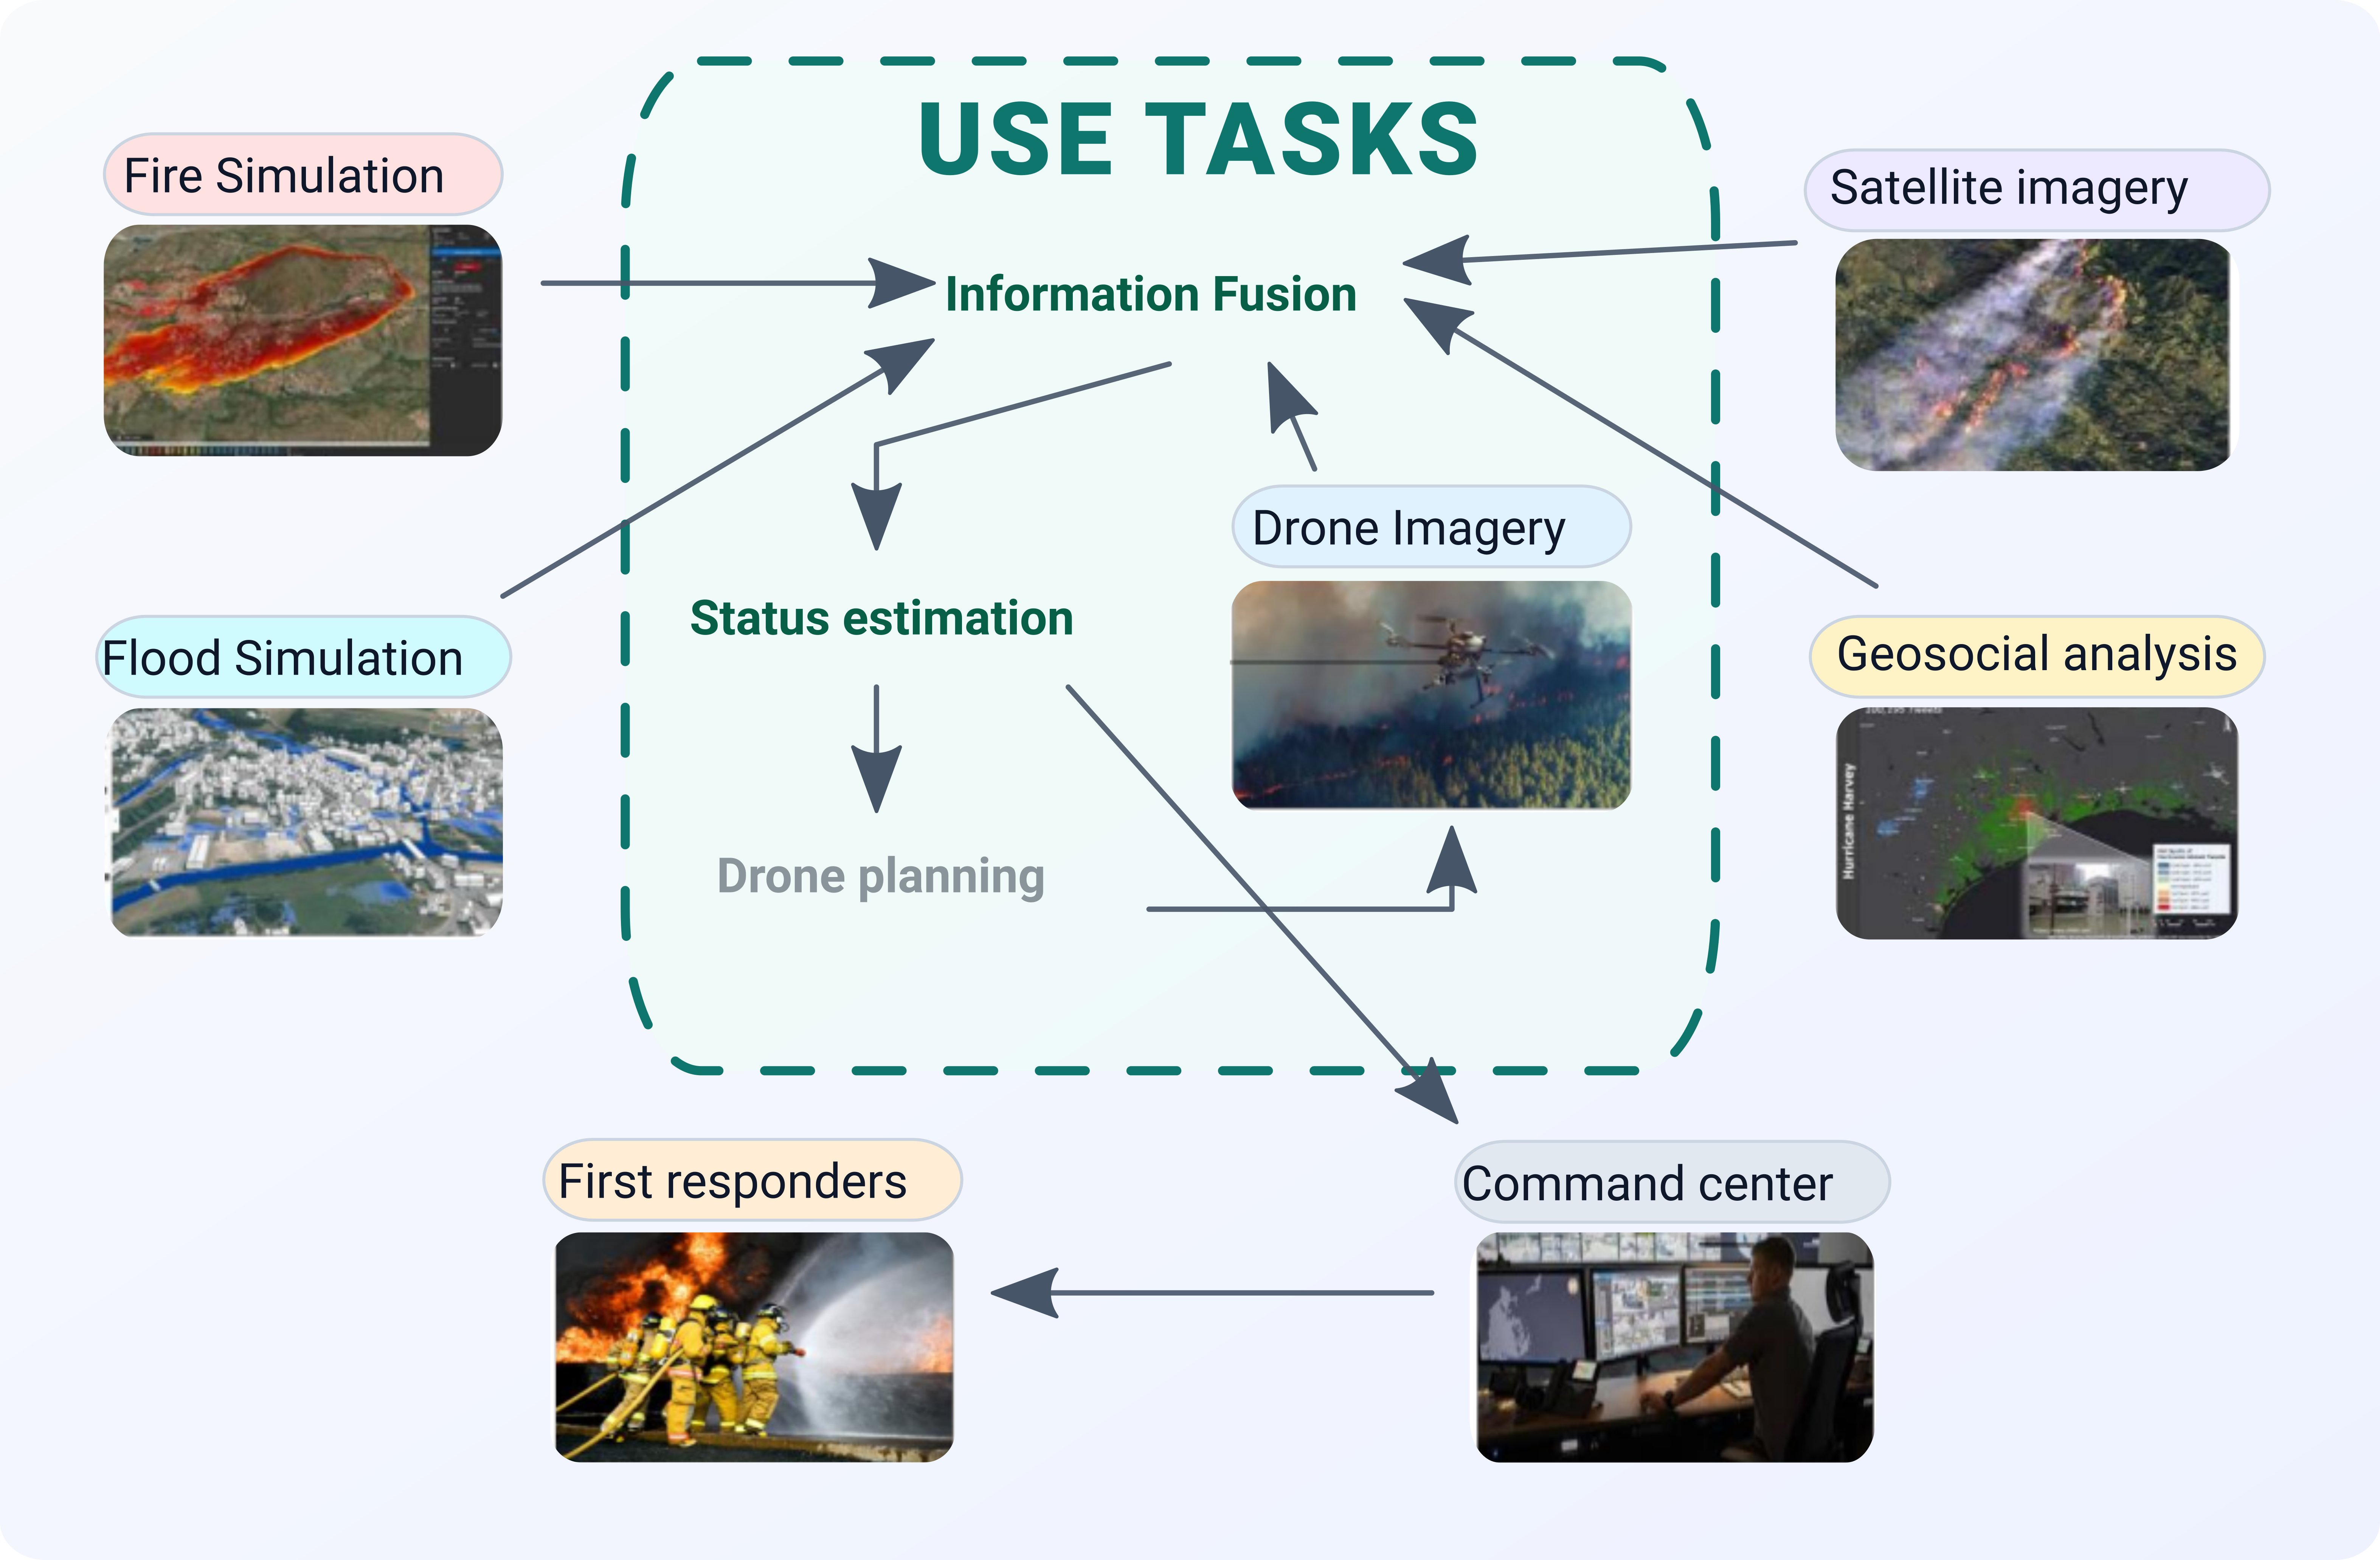
\includegraphics[width=\linewidth,height=0.72\textheight,keepaspectratio]{enhanced_end_to_end_scheme.png}
	\end{columns}
\end{frame}

\begin{frame}{Key challenges addressed by PDM-tech-05}
	\begin{itemize}
		\item \textbf{Heterogeneity:} mixing observations (UAV/satellite/geosocial) with model predictions
		\item \textbf{Asynchrony:} different refresh rates and latencies (seconds to hours).
		\item \textbf{Spatial mismatch:} different projections/resolutions \textrightarrow{} common reference grid
		\item \textbf{Uncertainty:} every source is imperfect; disagreement is normal.
		%    \item \textbf{Scalability:} update only where data overlap AOI; event-driven processing
		\item \textbf{Georeferencing:} UAV sensors + terrain $\Rightarrow$ spatial alignment is non-trivial.
		\item \textbf{Dynamics:} evolving hazard fronts and moving objects $\Rightarrow$ temporal consistency matters.
		%    \item \textbf{Actionability:} expose products via APIs and a web app to decision-support tools
	\end{itemize}
\end{frame}

\begin{frame}{How PDM-tech-05 connects to other TEMA technologies}
	\centering
	\includegraphics[width=0.98\linewidth,height=0.80\textheight,keepaspectratio]{INTERACTION_DIAGRAM.png}
\end{frame}



\begin{frame}{Two primary outputs: OGM and OPM}
	\small
	\begin{columns}[T,onlytextwidth]
		\column{0.48\textwidth}
		\begin{block}{Output 1: Occupancy Grid Map (OGM)}
			\begin{itemize}\itemsep0.35em
				\item Discretize the AOI into grid cells.
				\item Each cell stores a probability of occupancy:
				\begin{itemize}\itemsep0.2em
					\item \textbf{Flood OGM:} probability of water presence.
					\item \textbf{Fire OGM:} probability of fire/smoke/burnt area presence.
				\end{itemize}
				\item Updated asynchronously as new measurement \& prediction arrives.
			\end{itemize}
		\end{block}
		
		\column{0.48\textwidth}
		\begin{block}{Output 2: Object Presence Map (OPM)}
			\begin{itemize}\itemsep0.35em
				\item Tracks persons/vehicles in geodetic coordinates.
				\item Data association (Hungarian) + state estimation (Kalman).
				\item Produces stable trajectories and uncertainty..
			\end{itemize}
		\end{block}
		
		\vspace{0.4em}
		\begin{block}{Operational view (web app)}
			OGM + OPM are served as the evolving operational picture to the command center.
		\end{block}
	\end{columns}
\end{frame}

\begin{frame}{What the Information Fusion platform does}
	\begin{columns}[T,onlytextwidth]
		\column{1.0\textwidth}
		\begin{columns}[T,onlytextwidth]
			\column{0.33\textwidth}
			\tiny
			\begin{block}{PDM-tech-05: multimodal fusion framework for NDM}
				\begin{itemize}
					\tiny
					\item Select an Area of Interest (AOI) and a reference grid
					\item Ingest NGSI-LD entities (measurements +
					predictions) with timestamps and georeferencing metadata
					\item Fuse evidence probabilistically (event-driven
					updates).
					\item Maintain a persistent probabilistic state (\textbf{OGM} + \textbf{OPM})
					\item Publish updated products to the Digital Enabler / SmartDesk and trigger workflows
				\end{itemize}
			\end{block}
			\column{0.65\textwidth}
			\centering
			\begin{block}{Web app deployment view}
				\centering
				\includegraphics[width=1.0\linewidth,height=0.750\textheight,keepaspectratio]{web_app_diagram.png}
			\end{block}			
		\end{columns}
	\end{columns}
  	\begin{block}{Design principle}
  		\tiny
  		\textbf{Same engine across hazards $\Rightarrow$ Convert everything into consistent probabilities on a common spatial reference, then fuse.}
  	\end{block}
\end{frame}




\begin{frame}{Core engine: asynchronous occupancy-grid mapping}
  \begin{columns}[T,onlytextwidth]
    \column{0.46\textwidth}
      \begin{itemize}
        \item Maintain a grid of \textbf{log-odds} values (numerically stable)
        \item \textbf{Correction (sensor fusion):} apply an update when a new measurement arrives
        \item \textbf{Prediction (model-based):} propagate using predictions when measurements are absent
        \item Asynchrony is handled naturally (no need to wait for all sources).
      \end{itemize}
    \column{0.52\textwidth}
      \centering
      \includegraphics[width=\linewidth,height=0.66\textheight,keepaspectratio]{asyncapproach.png}
  \end{columns}
\end{frame}

% ============================================================
% OGM equations (consistent log-odds formalism)
% ============================================================
\begin{frame}{OGM formalism: probability and log-odds}
	\scriptsize
	\setlength{\abovedisplayskip}{2pt}
	\setlength{\belowdisplayskip}{2pt}
	
	Discretize the AOI into cells $m_i$ and maintain an occupancy probability $p_t(i)=P(m_i \text{ occupied at time } t)$.
	\vspace{0.35em}
	
	\begin{align*}
		\ell_t(i) &= \log \frac{p_t(i)}{1-p_t(i)} \qquad\text{(log-odds)}\\
		p_t(i) &= \sigma(\ell_t(i))=\frac{1}{1+e^{-\ell_t(i)}} \qquad\text{(logistic)}\\
		\ell_0(i) &= \log \frac{P(m_i)}{1-P(m_i)} \qquad\text{(prior; }P(m_i)=0.5\text{, so }\ell_0(i)=0\text{)}
	\end{align*}
	
	\begin{block}{Why log-odds?}
		Numerical stability and additive updates across asynchronous sources.
	\end{block}
\end{frame}

\begin{frame}{OGM fusion rule: Bayesian update in log-odds}
	\scriptsize
	\setlength{\abovedisplayskip}{2pt}
	\setlength{\belowdisplayskip}{2pt}
	
	For an incoming observation $z_t$ (from any source) and platform state $x_t$:
	\begin{align*}
		\ell_t(i)
		&= \ell_{t^-}(i) + \underbrace{\logit\!\big(P(m_i \mid z_t,x_t)\big)}_{\text{source evidence}} - \ell_0(i)
	\end{align*}
	
	\begin{block}{Interpretation}
		Each source produces a per-cell occupancy probability; we convert it to a log-odds increment and add it to the current map (subtracting the prior once to avoid double counting). In practice, we initialize $p_0(i)=0.5$ inside the AOI ($\ell_0(i)=0$), so the prior term vanishes; we keep $-\ell_0(i)$ to remain valid for non-uniform priors.
	\end{block}
\end{frame}


%\begin{frame}{OGM update: Bayesian log-odds fusion (asynchronous sources)}
%	\scriptsize
%	
%	\begin{block}{Occupancy grid cell $m_i$ (hazard present vs.\ absent)\\ Per-cell state}
%		\footnotesize
%		\vspace{0.6em}
%		Posterior occupancy probability after fusing measurements up to time $t$:
%		\[
%		p^t_i = P(m_i \mid z_{1:t}, x_{1:t}), \qquad
%		\ell^t_i = \log\frac{p^t_i}{1-p^t_i}, \qquad
%		\ell^0_i = \log\frac{p^0_i}{1-p^0_i}.
%		\]
%	\end{block}
%	
%	\vspace{-0.6em}
%	\begin{block}{Additive update (source $s$ arriving at time $t$)}
%		\footnotesize
%		Let $p^{t}_{i,s}\in(0,1)$ be the inverse-sensor-model output for cell $i$. Then:
%		\[
%		\ell^{t}_i = \ell^{t-}_i +
%		\left(\log\frac{p^{t}_{i,s}}{1-p^{t}_{i,s}} - \ell^0_i\right),
%		\qquad
%		p^{t}_i = \frac{1}{1+e^{-\ell^{t}_i}}.
%		\]
%	\end{block}
%\end{frame}


%\begin{frame}{OGM formalism: probability and log-odds}
%	\scriptsize
%	\begin{block}{Occupancy grid cell $m_i$ (hazard present vs.\ absent)}
%		\footnotesize
%		Posterior occupancy probability after fusing measurements up to time $t$:
%		\[
%		p_i^{t}=P(m_i \mid z_{1:t},x_{1:t}),\qquad
%		\ell_i^{t}=\log\frac{p_i^{t}}{1-p_i^{t}}.
%		\]
%		Prior:
%		\[
%		p_i^{0}=P(m_i),\qquad
%		\ell_i^{0}=\log\frac{p_i^{0}}{1-p_i^{0}}.
%		\]
%	\end{block}
%	
%	\vspace{-0.6em}
%	\begin{block}{Log-odds fusion update (conditionally independent sources)}
%		\footnotesize
%		For a new georeferenced measurement $z_t^s$ from source $s$:
%		\[
%		\ell_i^{t}
%		=\ell_i^{t-}+\Bigl(\log\frac{P(m_i\mid z_t^s,x_t)}{1-P(m_i\mid z_t^s,x_t)}-\ell_i^{0}\Bigr),
%		\]
%		then recover probability via $p_i^{t}=\sigma(\ell_i^{t})=(1+e^{-\ell_i^{t}})^{-1}$.
%	\end{block}
%\end{frame}


\begin{frame}{Fusion rule: measurements vs. predictions}
  \begin{columns}[T,onlytextwidth]
    \column{0.49\textwidth}
      \begin{block}{\textbf{Measurements} (UAV/satellite/geo-social) update the current OGM via inverse sensor models.}
        \begin{itemize}
          \item Convert raw outputs into a per-cell probability $p^{t}_{i,s}\in(0,1)$
          \item Add a log-odds increment $\delta\ell^{t}_{i,s} = \log\frac{p^{t}_{i,s}}{1-p^{t}_{i,s}}$
          \item Intuition: \textbf{high-confidence observations dominate locally}
        \end{itemize}
      \end{block}
    \column{0.49\textwidth}
      \begin{block}{{Predictions} (e.g., hydrodynamics, fire simulation)}
        \begin{itemize}
          \item Predictions provide \textbf{structured early evidence} over large areas
          \item Fuse with the current OGM via \textbf{logit pooling} (weighted combination in log-odds space)
          \item Intuition: \textbf{predictions guide} until observations override
        \end{itemize}
      \end{block}
  \end{columns}
\end{frame}

\begin{frame}{Flood measurement model: UAV flood segmentation}
	\scriptsize
	\begin{block}{Aggregation from high-resolution UAV raster to the OGM grid}
		For cell $i$, let $K_i$ be the set of georeferenced UAV pixels inside $i$ and $n_i=|K_i|$.
		\[
		\bar{s}^{\text{uav}}_i=\frac{1}{n_i}\sum_{k\in K_i} s^{\text{uav}}_k \in [0,1].
		\]
		Map the score to a measurement probability (clamp to $(\varepsilon,1-\varepsilon)$):
		\[
		p^{\text{uav}}_i = p^{\text{uav}}_{\min} + \bigl(p^{\text{uav}}_{\max}-p^{\text{uav}}_{\min}\bigr)\,\bar{s}^{\text{uav}}_i,
		\quad 0<p^{\text{uav}}_{\min}<p^{\text{uav}}_{\max}<1.
		\]
	\end{block}
	
	\vspace{-1.2em}
	\begin{block}{Log-odds increment and update}
		\footnotesize
		\[
		\delta\ell^{t}_{i,\text{uav}}=\log\frac{p^{\text{uav}}_i}{1-p^{\text{uav}}_i}-\ell_i^0,
		\qquad
		\ell^{t}_i=\ell^{t-}_i+\delta\ell^{t}_{i,\text{uav}}.
		\]
	\end{block}
	\vspace{-1.5em}
	\begin{block}{Notes}
		$\;p^{uav}_{\min},p^{uav}_{\max}$ encode trust in the segmentation (avoid overconfidence).
	\end{block}
\end{frame}


\begin{frame}{Flood measurement model: satellite flood extent}
  \scriptsize
  \begin{block}{Per-cell probability from a resampled satellite mask}
    Let $m^{\text{sat}}_i\in[0,1]$ be the resampled satellite mask value at cell $i$.
    For valid pixels:
    \[
      p^{\text{sat}}_i = m^{\text{sat}}_i \in (0,1),
      \qquad
      \delta\ell^{t}_{i,\text{sat}} = \log\frac{p^{\text{sat}}_i}{1-p^{\text{sat}}_i} -\ell_i^0,
      \qquad
      \ell^{t}_i=\ell^{t-}_i+\delta\ell^{t}_{i,\text{sat}}
    \]
    Cells outside the satellite swath (or invalid pixels) are not updated.
  \end{block}
  \vspace{0.4em}
  \begin{block}{Notes}
    Probabilities are clamped to $[\epsilon,1-\epsilon]$ (e.g., $\epsilon\approx 10^{-6}$) to avoid infinite log-odds.
  \end{block}
\end{frame}

\begin{frame}{Flood measurement model: geosocial hotspots}
  \scriptsize
  \begin{block}{From counts/ratios to measurement probability}
    Let $\tilde{c}_t(i)$ and $\tilde{r}_t(i)$ be normalized post count and activity ratio, and $w_c+w_r=1$.
    Define a hotspot score
    \[
      s^{\text{soc}}_t(i)=w_c\,\tilde{c}_t(i)+w_r\,\tilde{r}_t(i)\in[0,1],
    \]
    then convert to a probability
    \[
      p^{\text{soc}}_t(i)=\epsilon + (1-2\epsilon)\,s^{\text{soc}}_t(i),
      \qquad
      \delta\ell^{t}_{i,\text{soc}} = \log\frac{p^{\text{soc}}_t(i)}{1-p^{\text{soc}}_t(i)}-\ell_i^0,
      \qquad
      \ell^{t}_i=\ell^{t-}_i+\delta\ell^{t}_{i,\text{soc}}
    \]
  \end{block}
  \vspace{-0.4em}
  \begin{block}{Notes}
    Geosocial evidence is informative but noisy; weights are typically conservative compared to physical sources.
  \end{block}
\end{frame}

\begin{frame}{Flood prediction fusion: hydrodynamic depth (PDM-tech-02 / 3Di)}
  \scriptsize
  \begin{block}{Depth-to-probability mapping}
    Convert predicted water depth $h_i$ into occupancy probability via a logistic mapping:
    \begin{align*}
    	p^{hyd}_i &= \varepsilon + (1-2\varepsilon)\,\frac{1}{1+\exp\left(-\frac{h_i-h_{50}}{s}\right)} \\
    	\ell^{hyd}_i &= \log(\frac{p^{hyd}_i}{1-p^{hyd}_i}) -\ell_i^0
    \end{align*}
    \end{block}      
    \textbf{Logit pooling (weighted fusion in log-odds space):}
    \begin{align*}
    	\ell^{new}_i &= (1-\alpha_{hyd})\,\ell^{ogm}_i + \alpha_{hyd}\,\ell^{hyd}_i, \qquad p^{new}_i=\sigma(\ell^{new}_i)
    \end{align*}
    
    \begin{block}{Notes}
    	$\alpha_{hyd}\in[0,1]$ controls reliance on prediction vs.\ accumulated evidence.
    \end{block}
\end{frame}

%\begin{frame}{Fusing predictive outputs in a generic way}
%  \scriptsize
%  \begin{block}{Prediction as probabilistic evidence (example: fire arrival / flood simulation)}
%    For cell $i$, represent prediction as a pair of probabilities (hazard / no hazard):
%    \[
%      p^{\text{pred}}_i
%      = \frac{w_f\,p_f(i) + w_{nf}\,p_{nf}(i)}{w_f+w_{nf}},
%      \qquad w_f,w_{nf}>0.
%    \]
%    \vspace{-0.5em}
%    \begin{itemize}
%      \item \textbf{Flood:} $p_f(i)$ from model-derived inundation probability; $p_{nf}(i)=1-p_f(i)$.
%      \item \textbf{Fire:} $p_f(i)$ from arrival-time evidence (e.g., within a forecast horizon); $p_{nf}(i)=1-p_f(i)$.
%    \end{itemize}
%  \end{block}
%  \vspace{-0.6em}
%  \begin{block}{How it enters the OGM}
%    Use the same update interface as observations: convert $p^{\text{pred}}_i$ to log-odds and fuse; ; the same mechanism applies to floods and wildfires.
%  \end{block}
%\end{frame}

\begin{frame}{Extending beyond floods: fire occupancy (Maps4Fire)}
  \scriptsize
  \begin{block}{Fire-related measurements}
    \begin{itemize}
      \item UAV: \textit{FireSegmentation} and \textit{BurntSegmentation} (TFA-tech-06)
      \item Satellite: \textit{EOBurntArea} (TFA-tech-09)
      \item Geosocial: \textit{HotspotResult} (TFA-tech-11)
      \item Prediction: \textit{StandardArrivalTime} (PDM-tech-01)
    \end{itemize}
  \end{block}
  \vspace{-0.6em}
  \begin{block}{Example weighted combination (active fire vs. burnt evidence)}
    \[
      p_m(m_i)=w_{\text{fire}}\,p_{\text{fire}}(m_i)+w_{\text{burnt}}\,p_{\text{burnt}}(m_i),
      \qquad w_{\text{fire}}+w_{\text{burnt}}=1.
    \]
    This per-cell likelihood plugs into the same Bayesian occupancy update in log-odds space.
  \end{block}
\end{frame}

\begin{frame}{OPM: state, motion model, and asynchronous updates}
  \scriptsize
  {Geodetic state for each tracked object $k$ maintains a 6D state (geodetic position + velocity)}
    \[
      \mathbf{x}_{t,k}=\bigl[\lambda_{t,k}\;\;\phi_{t,k}\;\;h_{t,k}\;\;\dot{\lambda}_{t,k}\;\;\dot{\phi}_{t,k}\;\;\dot{h}_{t,k}\bigr]^{\top}.
    \] 
  \vspace{-0.6em}
  {Constant-velocity prediction transition:}    
    \[
    x_{t+1,k}=A x_{t,k} + w_t,\quad
    A=\begin{bmatrix}
    	1&0&0&\Delta t&0&0\\
    	0&1&0&0&\Delta t&0\\
    	0&0&1&0&0&\Delta t\\
    	0&0&0&1&0&0\\
    	0&0&0&0&1&0\\
    	0&0&0&0&0&1
    \end{bmatrix}
    \]
    {Prediction step:}
   	\[
   	\hat{x}_{t|t-1,k}=A\hat{x}_{t-1|t-1,k},\qquad
   	P_{t|t-1,k}=AP_{t-1|t-1,k}A^\top+Q
   	\]   	     
%  \vspace{-0.6em}
%  \begin{block}{Rationale}
%    Tracks persist even when detections are intermittent; uncertainty grows during prediction-only periods.
%  \end{block}
\end{frame}

\begin{frame}{OPM data association: gating and Hungarian assignment}
	\scriptsize
	\setlength{\abovedisplayskip}{2pt}
	\setlength{\belowdisplayskip}{2pt}
	
	For detection $j$ at position $p_{t,j}$ and predicted track position $\hat{p}_{t|t-1,k}$:
	\[
	d_{k,j}=d_{hav}(\hat{p}_{t|t-1,k},p_{t,j})
	\]
	
	Cost matrix for assignment:
	\[
	C_{k,j}=\alpha\,\frac{d_{k,j}}{r_{gate}}+\beta\,(1-c^{det}_{t,j})
	\]
	
	\begin{block}{Association}
		Apply gating ($d_{k,j}<r_{gate}$) then solve the assignment with the Hungarian algorithm.
	\end{block}
\end{frame}

\begin{frame}{OPM state correction: confidence-aware Kalman update}
	\scriptsize
	\setlength{\abovedisplayskip}{2pt}
	\setlength{\belowdisplayskip}{2pt}
	
	Measurement model (position):
	\[
	z_{t,j}=H x_{t,k}+v_t,\quad
	H=\begin{bmatrix}1&0&0&0&0&0\\0&1&0&0&0&0\\0&0&1&0&0&0\end{bmatrix}
	\]
	
	Confidence-aware measurement noise:
	\[
	R_{t,j}=\frac{1}{\max(c^{det}_{t,j},\varepsilon_c)}\,R_{base}
	\]
	
	Kalman update:
	\[
	S=HPH^\top+R,\quad K=PH^\top S^{-1},\quad
	\hat{x}_{t|t}=\hat{x}_{t|t-1}+K(z-H\hat{x}_{t|t-1})
	\]
\end{frame}

% ------------------------------------------------------------
% Information Fusion (PDM-tech-05) — University of Seville (USE)
% Case Study
% ------------------------------------------------------------
\GRVCsectionframe[assets/tema\_logo.png]{Historical and real-time trials}

{
	\GRVCsetprojectlogo{assets/tema_logo.pdf}


\begin{frame}<1-10>[t]{Trials timeline}
	\centering
	\vspace{-0.3em}
	\begin{tikzpicture}[x=0.36cm,y=0.80cm] % y scaled down to avoid clipping
		
		% Axis: start at Jun 2024 (x=-3), end at May 2027 (x=32)
		\draw[tlAxis] (-3,0) -- (32,0);
		
		% Minor monthly ticks
		\foreach \x in {-3,-2,...,32} {
			\draw[tlMinorTick] (\x,0.10) -- (\x,-0.10);
		}
		
		% Major ticks + month labels (jun added at -3; then sep/jan/may cadence)
		\foreach \x/\m in {-3/jun, 0/sep, 4/jan, 8/may, 12/sep, 16/jan, 20/may, 24/sep, 28/jan, 32/may} {
			\draw[tlMajorTick] (\x,0.16) -- (\x,-0.16);
			\node[tlMonth, above=2pt] at (\x,0.16) {\m};
		}
		
		% Year labels at January ticks
		\node[tlYear, below=7pt] at (4,0) {2025};
		\node[tlYear, below=7pt] at (16,0) {2026};
		\node[tlYear, below=7pt] at (28,0) {2027};
		
		% ---- Events (overlay animation) ----
		
		% June 2024 (new event) -> x = -3
		\only<1->{\TLBelow{-3}{-2.0}{tlOrange}{TLorange}{
				\textbf{Integration test}\\
				ENG\\
				Naples, Italy
		}}
		
		% Mar 2025 -> x = 6
		\only<2->{\TLAbove{6}{2.6}{tlOrange}{TLorange}{
				\textbf{Integration test}\\
				DLR-KN\\
				Munich, Germany
		}}
		
		% May 2025 -> x = 8
		\only<3->{\TLBelow{8}{-2.7}{tlBlue}{TLblue}{
				\textbf{Historical trial (Fire)}\\
				KAHY\\
				Kajaani, Finland
		}}
		
		% Jun 2025 -> x = 9
		\only<4->{\TLAbove{9}{1.4}{tlGreen}{TLgreen}{
				\textbf{Real-time experiment (Fire)}\\
				RAS\\
				Sardinia, Italy
		}}
		
		% Oct 2025 -> x = 13
		\only<5->{\TLBelow{13}{-1.4}{tlBlue}{TLblue}{
				\textbf{Historical trial (Floods)}\\
				D.MALIAN\\
				Mantoudi, Greece
		}}
		
		% Nov 2025 -> x = 14
		\only<6->{\TLAbove{14}{2.6}{tlBlue}{TLblue}{
				\textbf{Historical trial (Floods)}\\
				BRK\\
				Ahrtal region, Germany
		}}
		
		% Mar 2026 -> x = 18
		\only<7->{\TLBelow{18}{-2.7}{tlBlue}{TLblue}{
				\textbf{Historical trial (Fire)}\\
				RAS\\
				Sardinia, Italy
		}}
		
		% Jun 2026 -> x = 21
		\only<8->{\TLAbove{21}{1.5}{tlGreen}{TLgreen}{
				\textbf{Real-time experiment (Fire)}\\
				KAHY\\
				Kajaani, Finland
		}}
		
		% Sep 2026 -> x = 24
		\only<9->{\TLBelow{24}{-1.6}{tlGreen}{TLgreen}{
				\textbf{Real-time experiment (Floods)}\\
				BRK\\
				Ahrtal region, Germany
		}}
		
		% Oct 2026 -> x = 25
		\only<10->{\TLAbove{25}{2.6}{tlGreen}{TLgreen}{
				\textbf{Real-time experiment (Floods)}\\
				D.MALIAN\\
				Mantoudi, Greece
		}}
		
	\end{tikzpicture}
\end{frame}

\GRVCsectionframe[assets/tema\_logo.png]{CASE STUDY: AHRTAL FLOODS, Germany}

%\begin{frame}{Case study focus: floods (Ahrtal) as a demonstrator}
%  \begin{block}{Why a flood case study?}
%    The platform is hazard-agnostic, but floods provide a clear demonstration of fusing
%    predictions (hydrodynamics) with heterogeneous observations (UAV, satellite, geosocial).
%  \end{block}
%  \vspace{-0.2em}
%  \begin{itemize}
%    \item AOI defined as a polygon; OGM grid initialised with $p_i=0.5$ (unknown)
%    \item Sources fused asynchronously upon arrival:
%      \begin{itemize}
%        \item 3Di depth predictions \textrightarrow{} soft prior via logit pooling
%        \item UAV flood segmentation \textrightarrow{} high-resolution local corrections
%        \item Satellite flood extent \textrightarrow{} broader-area observational updates
%        \item Geosocial hotspots \textrightarrow{} human-centric weak evidence
%      \end{itemize}
%    \item Outputs delivered to decision-support tools: OGM (flood status) + OPM (persons/vehicles)
%  \end{itemize}
%\end{frame}

%%%%%%%%%%%%%%%%%%%%%%%%%%%%%%%%%%%%%%%%%%%%%%
\begin{frame}{Case study setup: AOI and common grid}
	\begin{columns}[T,onlytextwidth]
		\column{0.55\textwidth}
		\small
		\begin{itemize}\itemsep0.55em
			\item AOI defined as a polygon; discretized into an OGM grid.
			\item Initialization: $p_0(i)=0.5$ (maximum uncertainty) inside AOI.
			\item Asynchronous fusion as sources arrive: 3Di prediction, UAV segmentation, satellite extent, geo-social hotspots.
			\item Objective: progressively refine the flood probability map (FPM).
		\end{itemize}
		\column{0.43\textwidth}
		\centering
		\includegraphics[width=\linewidth,height=0.75\textheight,keepaspectratio]{assets/aoi_satellite_with_bw_colorbar.png}
	\end{columns}
\end{frame}


\begin{frame}{What gets fused in the OGM (inputs + roles)}
	\small
	\begin{block}{Evidence roles (hazard-agnostic pattern)}
		\begin{itemize}\itemsep0.35em
			\item \textbf{Hydrodynamics}: early spatial structure (physics-informed), but predictive uncertainty.
			\item \textbf{Satellite}: wide-area observational correction (coarser + time offsets).
			\item \textbf{UAV segmentation}: local, high-resolution refinement on demand (small footprint, high fidelity).
			\item \textbf{Geosocial}: additive human-centric confirmation; may be spatially coarse.
		\end{itemize}
	\end{block}
	
	\begin{block}{Key takeaway}
		OGM/FPM integrates all sources on a common grid using probabilistic updates; it does not treat any source as ground truth.
	\end{block}
\end{frame}

\begin{frame}{3Di prediction: depth $\rightarrow$ flood probability prior}
	\begin{columns}[T,onlytextwidth]
		\column{0.48\textwidth}
		\centering
		\includegraphics[width=\linewidth,height=0.65\textheight,keepaspectratio]{assets/3di_depth.png}
		\vspace{0.3em}
		\scriptsize Predicted water depth (3Di)
		\column{0.48\textwidth}
		\centering
		\includegraphics[width=\linewidth,height=0.65\textheight,keepaspectratio]{assets/3di_probability.png}
		\vspace{0.3em}
		\scriptsize Mapped flood probability $p^{hyd}_i$
	\end{columns}
	\vspace{-0.2em}
	\footnotesize
	\begin{itemize}\itemsep0.25em
		\item Prediction is fused conservatively (logit pooling) to avoid over-committing early.
		\item Sets the initial large-scale structure before high-resolution observations arrive.
	\end{itemize}
\end{frame}

\begin{frame}{UAV flood segmentation: image $\rightarrow$ mask $\rightarrow$ georeferenced evidence}
	\centering
	% --- Top row: three-stage visual narrative ---
	\includegraphics[width=0.32\linewidth,height=0.30\textheight,keepaspectratio]{assets/uav_captured_img.jpg}\hfill
	\includegraphics[width=0.32\linewidth,height=0.30\textheight,keepaspectratio]{assets/Flood_DJI_20211023131552_0001_Z_A.jpg}\hfill
	\includegraphics[width=0.32\linewidth,height=0.30\textheight,keepaspectratio]{assets/uav_geotiff_on_satellite.jpg}
	
	\vspace{0.35em}
	\begin{columns}[T,onlytextwidth]
		\column{0.56\textwidth}
		\small
		\begin{itemize}\itemsep0.4em
			\item UAV RGB imagery segmented into flood / non-flood.
			\item Mask is \textbf{georeferenced} onto the AOI (pose + DEM).
			\item Produces local, high-resolution observational evidence to correct the map.
		\end{itemize}
		\column{0.42\textwidth}
		\centering
		\includegraphics[width=\linewidth,height=0.40\textheight,keepaspectratio]{assets/uav_segmentation.png}
	\end{columns}
\end{frame}

\begin{frame}{Satellite flood extent: wide-area observational update}
	\begin{columns}[T,onlytextwidth]
		\begin{column}{0.38\textwidth}
			\small
			\begin{itemize}\itemsep0.4em
				\item Satellite surface-water extent product (probabilistic raster).
				\item Reprojected + resampled to the \textbf{5 m FPM grid}.
				\item Broad coverage complements UAV footprint; corrects regional mismatches.
			\end{itemize}
		\end{column}
		\begin{column}{0.60\textwidth}
			\includegraphics[width=\linewidth,height=0.66\textheight,keepaspectratio]{assets/satellite_aoi.png}		
		\end{column}
	\end{columns}
\end{frame}

%\begin{frame}{UAV flood segmentation}
%	\centering	
%	% ---------- Top row: 3 images ----------
%	\begin{minipage}[t]{0.32\linewidth}
%		\centering
%		\includegraphics[height=0.26\textheight,keepaspectratio]{assets/uav_captured_img.jpg}
%	\end{minipage}\hfill
%	\begin{minipage}[t]{0.32\linewidth}
%		\centering
%		\includegraphics[height=0.26\textheight,keepaspectratio]{assets/Flood_DJI_20211023131552_0001_Z_A.jpg}
%	\end{minipage}\hfill
%	\begin{minipage}[t]{0.32\linewidth}
%		\centering
%		\includegraphics[height=0.26\textheight,keepaspectratio]{assets/uav_geotiff_on_satellite.jpg}
%	\end{minipage}
%	
%	\vspace{0.5em}
%	
%	% ---------- Bottom: text + 4th image ----------
%	\begin{columns}[T,onlytextwidth]
%		\begin{column}{0.75\textwidth}
%			\small
%			\begin{itemize}\itemsep0.35em
%				\item UAV RGB imagery segmented into flood / non-flood.
%				\item Mask is \textbf{georeferenced} onto the AOI (DEM + pose).
%				\item Produces local, high-resolution observational evidence.
%			\end{itemize}
%		\end{column}
%		\begin{column}{0.22\textwidth}
%		\end{column}
%	\end{columns}
%\end{frame}
%
%
%\begin{frame}{UAV evidence on the map: local probabilities}
%	\begin{columns}[T,onlytextwidth]
%		\begin{column}{0.49\textwidth}
%			\small
%			\begin{itemize}\itemsep0.4em
%				\item UAV flood segmentation converted to per-cell likelihoods.
%				\item Interpreted as \textbf{local flood probabilities} on the FPM grid.
%				\item Key role: \textbf{boundary sharpening} and local corrections.
%			\end{itemize}
%		\end{column}
%		\begin{column}{0.49\textwidth}
%			\centering
%			\includegraphics[height=0.5\textheight,keepaspectratio]{assets/uav_segmentation.png}
%		\end{column}
%	\end{columns}
%\end{frame}

\begin{frame}{Geosocial hotspots: human-centric evidence (and limitations)}
	\begin{columns}[T,onlytextwidth]
		\begin{column}{0.45\textwidth}
			\small
			\begin{itemize}\itemsep0.4em
				\item Posts aggregated into hotspot cells (counts, activity, stats).
				\item Converted into a measurement likelihood $p^{soc}_t(i)$.
				\item Ahrtal limitation: AOI falls in a \textbf{single hotspot cell} $\Rightarrow$ coarse spatial signal.
			\end{itemize}
		\end{column}
		
		\begin{column}{0.52\textwidth}
			\centering
			\includegraphics[width=\linewidth,height=0.34\textheight,keepaspectratio]{assets/geosocial_raw.png}\par
			\vspace{0.5em}
			\includegraphics[width=\linewidth,height=0.34\textheight,keepaspectratio]{assets/geosocial_pm.png}
		\end{column}
	\end{columns}
\end{frame}


\begin{frame}{Qualitative evolution: the FPM sharpens as evidence arrives}
	\centering
	\setlength{\tabcolsep}{3pt}
	\renewcommand{\arraystretch}{1.0}
	\begin{tabular}{cc}
		\includegraphics[width=0.48\linewidth,height=0.33\textheight,keepaspectratio]{assets/fpm_after_3di_greys_inset.png} &
		\includegraphics[width=0.48\linewidth,height=0.33\textheight,keepaspectratio]{assets/fpm_before_geosocial_zoom_cells.png} \\
		\includegraphics[width=0.48\linewidth,height=0.33\textheight,keepaspectratio]{assets/fpm_after_geosocial_zoom_cells.png} &
		\includegraphics[width=0.48\linewidth,height=0.33\textheight,keepaspectratio]{assets/final_fpm_multimodal_fusion.png}
	\end{tabular}	
%	\vspace{0.35em}
%	\footnotesize
%	\vspace{0.4em}
	\footnotesize
	\begin{itemize}\itemsep0.2em
		\footnotesize
		\item Predictions provide early structure; observations refine boundaries and correct local mismatches.
		\item Geosocial contribution is deliberately moderate but visible in the inset.
	\end{itemize}
\end{frame}


\begin{frame}{Quantitative evolution: uncertainty reduction and change detection}
	\begin{columns}[T,onlytextwidth]
		\column{0.54\textwidth}
		\small
		\begin{itemize}\itemsep0.6em
			\item Track the entropy of the flood probability map (FPM) to quantify confidence gains.
			\item Use map-to-map changes ($\Delta$) to detect when new evidence meaningfully updates the picture.
			\item In Ahrtal, the strongest corrections coincide with UAV and satellite arrivals.
		\end{itemize}
		\column{0.44\textwidth}
		\centering
		\includegraphics[width=\linewidth,height=0.75\textheight,keepaspectratio]{assets/fpm_entropy_delta.png}
	\end{columns}
\end{frame}

%\begin{frame}{Temporal behavior: responsiveness + stability}
%	\begin{columns}[T,onlytextwidth]
%		\begin{column}{0.42\textwidth}
%			\small
%			\begin{itemize}\itemsep0.4em
%				\item Metrics computed over published FPMs (5-min intervals).
%				\item $\Delta(t)$ spikes when strong evidence arrives, then $\rightarrow 0$ (convergence).
%				\item $H(t)$ decreases as uncertainty reduces.
%			\end{itemize}
%		\end{column}
%		\begin{column}{0.58\textwidth}
%			\centering
%			% fpm_entropy_delta.png
%			\includegraphics[width=0.80\textheight,keepaspectratio]{assets/fpm_entropy_delta.png}
%		\end{column}
%	\end{columns}
%\end{frame}


%\begin{frame}{Cross-modality consistency (internal agreement with final FPM)}
%	\small
%	\begin{block}{Why this metric?}
%		Dense external ground truth is limited; we quantify how the fused FPM aligns with each modality on its support.
%	\end{block}
%	
%	\vspace{-0.2em}
%	\centering
%	\footnotesize
%	\begin{tabular}{lrrr}
%		\hline
%		Source $s$ & $|I_s|$ [cells] & $D_s$ & $A_s$ [\%] \\
%		\hline
%		UAV segmentation          & 326    & 0.05 & 97 \\
%		Satellite SWIM product    & 58{,}789 & 0.12 & 90 \\
%		Hydrodynamic (3Di)        & 58{,}789 & 0.18 & 85 \\
%		Geosocial hotspots        & 58{,}789 & 0.35 & 52 \\
%		\hline
%	\end{tabular}
%	
%	\vspace{0.6em}
%	\small
%	\begin{itemize}\itemsep0.3em
%		\item UAV aligns best (high local fidelity on its footprint).
%		\item Satellite moderate (observational but coarser / time offset).
%		\item Hydrodynamics lower (predictive uncertainty).
%		\item Geosocial lowest (coarse spatial support in Ahrtal).
%	\end{itemize}
%\end{frame}


\begin{frame}{OPM setup: detections $\rightarrow$ georeferenced observations $\rightarrow$ tracker}
	\small
	\begin{itemize}\itemsep0.45em
		\item UAV person/vehicle detections are georeferenced to $(\lambda,\phi,h)$ with confidence.
		\item Multi-object mode: \textbf{gating + Hungarian assignment} for association.
		\item State estimation: \textbf{6D geodetic Kalman filter} (prediction-only during detection gaps).
		\item Discontinuity rule: reject updates when prediction--measurement discrepancy exceeds \textbf{$r_{\mathrm{FPM}}=5$ m} (aligned with OGM resolution).
	\end{itemize}
\end{frame}


\begin{frame}{Tracking under missed detections: gaps and continuity}
	\begin{columns}[T,onlytextwidth]
		\begin{column}{0.45\textwidth}
			\centering
			\includegraphics[width=0.80\textheight,keepaspectratio]{assets/measurement_availability.png}
		\end{column}
		\begin{column}{0.50\textwidth}
			\includegraphics[width=0.80\textheight,keepaspectratio]{assets/4_longitude_over_time.png}
		\end{column}
	\end{columns}
	
	\vspace{0.4em}
	\small
	\begin{itemize}\itemsep0.25em
		\item During gaps: prediction-only propagation; filtered state remains continuous.
		\item When detections return: correction pulls the trajectory back toward measurements.
	\end{itemize}
\end{frame}

%\begin{frame}{Tracking diagnostics: longitude/latitude/altitude over time}
%	\begin{columns}[T,onlytextwidth]
%		\begin{column}{0.42\textwidth}
%			\small
%			\begin{itemize}\itemsep0.4em
%				\item Filtered estimate is smooth yet responsive.
%				\item During measurement gaps: filtered $\approx$ prediction.
%				\item Altitude remains nearly constant (plausible pedestrian motion + terrain).
%			\end{itemize}
%		\end{column}
%		\begin{column}{0.58\textwidth}
%			\centering
%			% Fig.16 is on page 27 (middle-lower). Crop to the three small plots region.
%			\paperfig{27}{\linewidth}{1.0cm 7.2cm 1.0cm 8.6cm}
%			\vspace{-0.5em}
%			{\scriptsize Fig. 16: Longitude, latitude, altitude over 30 frames.}
%		\end{column}
%	\end{columns}
%\end{frame}


%\begin{frame}{Consistency diagnostics: residuals bounded by map resolution}
%	\begin{columns}[T,onlytextwidth]
%		\begin{column}{0.45\textwidth}
%			\small
%			\begin{itemize}\itemsep0.4em
%				\item Prediction--measurement distance and innovation magnitude stay within bounds.
%				\item Reset threshold corresponds to \textbf{$r_{\mathrm{FPM}}=5$ m}.
%				\item Prevents spurious long-range stitching across gaps.
%			\end{itemize}
%		\end{column}
%		\begin{column}{0.55\textwidth}
%			\centering
%			% Fig.17 is on page 28 (top). Crop to the top plots.
%			\paperfig{28}{\linewidth}{1.0cm 14.2cm 1.0cm 2.0cm}
%			\vspace{-0.5em}
%			{\scriptsize Fig. 17: Distance and innovation; threshold at 5 m.}
%		\end{column}
%	\end{columns}
%\end{frame}

%\begin{frame}{3D trajectory: what the OPM output looks like}
%	\begin{columns}[T,onlytextwidth]
%		\begin{column}{0.42\textwidth}
%			\small
%			\begin{itemize}\itemsep0.4em
%				\item Kalman filtering reduces high-frequency georeferencing noise.
%				\item Maintains continuity through intermittent detections.
%				\item Produces a compact movement summary for decision support.
%			\end{itemize}
%		\end{column}
%		\begin{column}{0.58\textwidth}
%			\centering
%			% Fig.18 is on page 28 (middle). Crop to the 3D plot region.
%			\paperfig{28}{\linewidth}{1.0cm 6.0cm 1.0cm 9.4cm}
%			\vspace{-0.5em}
%			{\scriptsize Fig. 18: 3D tracked trajectory (meas/pred/filtered).}
%		\end{column}
%	\end{columns}
%\end{frame}
%
%
%\begin{frame}{Case study takeaways: what it proves about Information Fusion}
%	\small
%	\begin{itemize}\itemsep0.45em
%		\item \textbf{OGM/FPM}: reacts strongly when new modalities arrive (large $\Delta(t)$), then stabilizes (convergence).
%		\item \textbf{Multimodal behavior}: predictions provide structure; observations (especially UAV) refine boundaries and correct local mismatches.
%		\item \textbf{OPM}: coherent tracking under intermittent detections; consistency enforced at \textbf{5 m} map resolution.
%	\end{itemize}
%	
%	\vspace{0.6em}
%	\centering
%	\begin{columns}[T,onlytextwidth]
%		\begin{column}{0.33\textwidth}
%			\paperfig{24}{\linewidth}{1.0cm 12.2cm 1.0cm 2.0cm}\\[-0.4em]
%			{\scriptsize Final FPM (Fig. 12)}
%		\end{column}
%		\begin{column}{0.33\textwidth}
%			\paperfig{25}{\linewidth}{1.0cm 16.0cm 1.0cm 2.0cm}\\[-0.4em]
%			{\scriptsize Temporal metrics (Fig. 13)}
%		\end{column}
%		\begin{column}{0.33\textwidth}
%			\paperfig{28}{\linewidth}{1.0cm 10.0cm 1.0cm 6.0cm}\\[-0.4em]
%			{\scriptsize 3D OPM track (Fig. 18)}
%		\end{column}
%	\end{columns}
%\end{frame}
% ============================================================
% Wrap-up
% ============================================================
\begin{frame}{Key takeaways}
	\small
	\begin{itemize}\itemsep0.6em
		\item \textbf{Generic platform} for NDM: consistent handling of heterogeneous, asynchronous evidence.
		\item \textbf{Two operational products:} OGM (Flood/Fire status) and OPM (multi-object tracking).
		\item \textbf{Robust fusion:} Bayesian log-odds updates for measurements + logit pooling for predictions.
		\item \textbf{Operationalization:} event-driven services + web app cockpit + NGSI-LD interoperability.
		\item \textbf{USE loop:} Fusion $\rightarrow$ Drone planning $\rightarrow$ Drone acquisition $\rightarrow$ Fusion.
	\end{itemize}
\end{frame}
%%%%%%%%%%%%%%%%%%%%%%%%%%%%%%%%%%%%%%%%%%%%%%

\GRVCclearprojectlogo
} 
\GRVCsectionframe[assets/grvc_logo.png]{\Large \textbf{Thank you for attending, Questions?}}
\end{document}
